% !TEX root = ../main.tex
\begin{figure}[t]
  \centering
  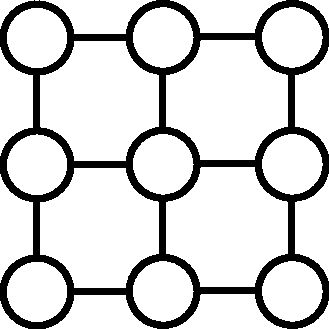
\includegraphics[height=0.2\paperheight]{fig/graphical-model-ising.pdf}
  \caption[Ising model as a probabilistic model]{
  \textbf{The Ising model is a probabilistic model used in statistical physics.} The nodes in this probabilistic graphical model represent random variables, and the edges in the graph represent relationships between neighboring random variables. In this Ising model there are nine random variables variables $\mbz = \{z_1, z_2, \ldots, z_9\}$ represented by nodes and the edges connecting two nodes indicate that those random variables interact in the energy function of the model $E(\mbz)$.}
  \label{fig:graphical-model-ising}
\end{figure}